
\documentclass[12pt]{article}
\usepackage{amsmath}
\DeclareMathOperator*{\argmin}{arg\,min} % thin space, limits underneath in displays
\DeclareMathOperator*{\argmax}{arg\,max} % thin space, limits underneath in displays
\newtheorem{thm}{Theorem}
\usepackage{amssymb}
\usepackage{amsfonts}
\usepackage{mathrsfs}
\usepackage{bm}
\usepackage{indentfirst}
\setlength{\parindent}{0em}
\usepackage[margin=1in]{geometry}
\usepackage{graphicx}
\usepackage{setspace}
\doublespacing
\usepackage[flushleft]{threeparttable}
\usepackage{booktabs,caption}
\usepackage{float}
\usepackage{graphicx}
\usepackage[sort,comma]{natbib}
\usepackage[hidelinks]{hyperref}

\usepackage{import}
\usepackage{xifthen}
\usepackage{pdfpages}
\usepackage{transparent}

\newcommand{\incfig}[1]{%
\def\svgwidth{\columnwidth}
\import{./figures/}{#1.pdf_tex}
}




\title{}
\author{}
\date{}


\begin{document}

Now introduce two models that resemble the Solow model but in which the dynamics of
economic aggregates are determined by decisions at the microeconomic level.

In this Note, we introduce the Ramsey-Cass-Koopmans model. It avoids all mkt 
imperfections and all inssues raised by heterogeneous HHs nd links among generations.

In the next Note, we introduce Overlapping-generations model developed by Diamond 
(1965).
The key difference of Diamond's model is that it assumes continual entry of new HHs
into the economy.






\section{Assumptions}

General Assumptions:

1. Labor and technology grow at an exogenous growth rate $ n $ and $ g $.

2. Competitive firms rent capital and hire labor to produce.

3. A fixed number of infinitely lived HHs.



\subsection{Firms}

Production Fn: CRTS
\begin{equation*}
Y = F(K,AL)
\end{equation*}


Capital accumulation is determined by output and consumption, same as the Solow model. 
However, we now assume {\textbf {No depreciation}}.

\begin{equation*}
\dot{K}(t) = Y(t) - \xi(t)
\end{equation*}

\begin{align*}
		\xi&: \text{ total consumption. }\\
		C &: \text{ consumption per person. }\\
		c &: \text{ consumption per effective labor. }
\end{align*}



\subsection{Households}

1. The size of each HH grows at rate $ n $. 

2. Each member of the HH supplies 1 unit of labor.

3. HH's income goes to consumption and saving.

\begin{align*}
H &: \text{ the number of HHs }\\
K(0)&: \text{ initial capital in the economy }\\
\frac{K(0)}{H} &: \text{ initial capital held by each HH }\\
C(t) &: \text{ consumption per person }\\
L(t) &: \text{ total population in the economy }\\
\frac{L(t)}{H} &: \text{ the number of members of each HH }\\
u(C(t))\frac{L(t)}{H} &: \text{ HH's utility at time $ t $ }\\
\rho &: \text{ discount rate. HH is impatient if $ \rho $ is large.}
\end{align*}

A discrete model:
\begin{equation*}
U = \sum\limits_{t = 0} ^\infty \left( \frac{1}{1 + \rho} \right) ^{t}
u(C(t))\frac{L(t)}{H}
\end{equation*}



Convert it to a continuous model:
\begin{equation*}
U = \int_{t = 0}^{\infty } e^{ - \rho t}u(C(t))\frac{L(t)}{H}dt
\end{equation*}
The utility fn:
\begin{equation*}
u(C(t)) = \frac{C(t)^{1 - \theta}}{1 - \theta}, \quad \theta > 0, \quad
\rho - n - (1 - \theta)g > 0
\end{equation*}
This function form is needed for the convergence (to the SS). It is known as 
{\textbf {constant-relative-risk-aversion}} (CRRA) utility.
The coefficient of relative risk aversion ($  - \frac{C u''}{u'} $) is $ \theta $,
and is independent from $ C $.

When $ \theta $ is smaller, MU falls more slowly (check $ u'' $) as $ C $ rises. So
HH is more willing to allow consumption to vary over time.

When $ \theta \rightarrow 1 $, it becomes $ u(C) = \ln C $

Utility will not explode to infinity because of  $ \rho - n - (1 - \theta)g > 0 $.






\section{Model}
\subsection{Firms}

No depreciation, so capital earn its MPK.
\begin{equation*}
r(t) = f'(k(t))
\end{equation*}

The MPL is 
\begin{equation*}
		\frac{\partial F(K, AL) }{\partial L } = A[f(k) - kf'(k)]
\end{equation*}
\noindent\fbox{%
\parbox{\textwidth}{%
Proof:
\begin{align*}
\frac{\partial F(K,AL) }{\partial L }&= \frac{\partial AL F(\frac{K}{AL},1) }
{\partial L }\\
&= A \left[ F(\frac{K}{AL},1) + L F'(\frac{K}{AL},1)( - \frac{K}{AL^{2}}) \right] \\
&= A \left( f(k) - Lf'(k)\frac{k}{L} \right), \quad k = \frac{K}{AL} \\
&= A [ f(k) - kf'(k)]
\end{align*}
}%
}\\



So the real wage, $ W(t) $, is 
\begin{equation*}
		W(t) = MPL = A(t)[f(k(t)) - k(t)f'(k(t))]
\end{equation*}

The wage per unit of effective labor is
\begin{equation*}
w(t) =f(k) - kf'(k) =  f(k(t)) - k(t)f'(k(t))
\end{equation*}


\subsection{Household Budget constraint}



To allow $ r $ changing over time, we define 
\begin{equation*}
R(t) = \int_{\tau = 0}^{t} r(\tau)d \tau
\end{equation*}

One unit of investment at time 0 yields $ e^{R(t)} $ units. It shows the continuously
compounding interest over the period [0,t].

The value of one unit of output at time $ t $ in terms of output at time 0 is
$ e^{ - R(t)} $. If $ r $ is constant, $ R(t) = r t $


 $  $.
\begin{align*}
\text{ Labor income for a HH }&:W(t)\frac{L(t)}{H}\\
\text{ Consumption expenditure for a HH }&: C(t)\frac{L(t)}{H}\\
\text{ initial wealth }&: \frac{1}{H} \text{ of total wealth at time 0 }
= \frac{K(0)}{H}
\end{align*}



{\textbf {HH BC:}}

\begin{equation}
\label{eqn:HHBC}
\int_{t = 0}^{\infty } e^{ - R(t)}C(t)\frac{L(t)}{H}d t \le 
\frac{K(0)}{H} + \int_{t = 0}^{\infty } e^{ - R(t)} W(t)\frac{L(t)}{H} d t
\end{equation}

{\textbf {Transversality Condition:}}

We can rewrite the BC (equation \eqref{eqn:HHBC}) with a specific timestamp $ s $
\begin{equation}
		\label{eqn:lim BC}
\lim_{s \to \infty}\left[ 
		\frac{K(0)}{H} + \int_{t = 0}^{s} e^{ - R(t)}[W(t) - C(t)]\frac{L(t)}{H}d t
\right] \ge  0
\end{equation}


Recall that $ e^{R(s)} $ measures the continuously compunding return from time 0 to
time $ s $.
Therefore, with your initial wealth of $ \frac{K(0)}{H} $ at time 0, this initial 
wealth at period $ s $ would become $ e^{R(s)} \frac{K(0)}{H} $.

So, HH's wealth at period $ s $, $ \frac{K(s)}{H} $, would be:
\begin{align*}
\frac{K(s)}{H} &= e^{R(s)}
\left[ 
		\frac{K(0)}{H} + \int_{t = 0}^{s} e^{ - R(t)}[W(t) - C(t)]\frac{L(t)}{H}d t
\right] 
\end{align*}

Now, we can rewrite the BC in equation \eqref{eqn:lim BC} in this form,
\begin{equation*}
\lim_{s \to \infty}e^{ - R(s)}\frac{K(s)}{H} \ge 0
\end{equation*}
This is the transversality condition.


\subsection{Household's Maximization Problem}

We use $ c(t) $ for consumption per effective worker. Recall $ C(t) $ is consumption
per worker, therefore, 
\begin{align*}
c(t) &= \frac{C(t)}{A(t)}\\
C(t) &= A(t)c(t)
\end{align*}

Now we can rewrite the utility function:
\begin{align*}
u(C(t)) = \frac{C(t)^{1 - \theta}}{1 - \theta}
&= \frac{[A(t)c(t)]^{1 - \theta}}{1 - \theta}\\
&= \frac{[A(0)e^{gt}]^{1 - \theta}c(t)^{1 - \theta}}{1 - \theta}\\
&= A(0)^{1 - \theta}e^{gt(1 - \theta)}\frac{c(t)^{1 - \theta}}{1 - \theta}
\end{align*}
Note, 
\begin{equation*}
A(t) = \lim_{n \to \infty}A(0)(1 + \frac{g}{n})^{nt} = A(0)e^{gt}.
\end{equation*}


Now plug $ u(C(t)) $ into lifetime utility function:
\begin{align*}
U &= \int_{t = 0}^{\infty } e^{ - \rho t}u(C(t))\frac{L(t)}{H}d t\\
&= \int_{t = 0}^{\infty } e^{ - \rho t}
\left[ 
A(0)^{1 - \theta}e^{gt(1 - \theta)}\frac{c(t)^{1 - \theta}}{1 - \theta}
\right] 
\frac{L(0)e^{nt}}{H}d t\\
&= A(0)^{1 - \theta}\frac{L(0)}{H} \int_{t = 0}^{\infty } 
e^{ - \rho t} e^{gt(1 - \theta)} e^{nt}\frac{c(t)^{1 - \theta}}{1 - \theta}d t\\
&= B \int_{t = 0}^{\infty } e^{ - \beta t} \frac{c(t)^{1 - \theta}}{1 - \theta}d t
\end{align*}
where
\begin{align*}
B &= A(0)^{1 - \theta} \frac{L(0)}{H}\\
\beta &= \rho - n - (1 - \theta)g > 0
\end{align*}


Now we convert the HH BC to an ``per effective worker form":

\begin{align*}
\int_{t = 0}^{\infty } e^{ - R(t)}C(t)\frac{L(t)}{H}d t &\le 
\frac{K(0)}{H} + \int_{t = 0}^{\infty } e^{ - R(t)}W(t)\frac{L(t)}{H}d t\\
c(t)&= \frac{C(t)}{A(t)}\\
k(0)&= \frac{K(0)}{A(0)L(0)}\\
w(t)&= \frac{W(t)}{A(t)}\\
\int_{t = 0}^{\infty } e^{ - R(t)}c(t)\frac{A(t)L(t)}{H}d t & \le 
k(0)\frac{A(0)L(0)}{H} + \int_{t = 0}^{\infty } e^{ - R(t)}w(t)\frac{A(t)L(t)}{H}d t\\
\int_{t = 0}^{\infty } e^{ - R(t)}c(t)\frac{A(0)L(0)e^{(g + n)t}}{H}d t & \le 
k(0)A(0)L(0) + \int_{t = 0}^{\infty } e^{ - R(t)}w(t)\frac{A(0)L(0)e^{(g + n)t}}{H}d t\\
\int_{t = 0}^{\infty } e^{ - R(t) + (g + n)t}c(t)d t & \le 
k(0) + \int_{t = 0}^{\infty } e^{ - R(t) + (g + n)t}w(t)d t
\end{align*}




{\textbf {Lagragian equation:}}

\begin{align*}
\mathscr{L} =& B \int_{t = 0}^{\infty } e^{ - \beta t} \frac{c(t)^{1 - \theta}}
{1 - \theta} dt\\
& + \lambda \left[ 
k(0) + \int_{t = 0}^{\infty } e^{ - R(t) + (g + n)t}w(t)d t  - 
\int_{t = 0}^{\infty } e^{ - R(t) + (g + n)t}c(t) d t
\right] 
\end{align*}

{\textbf {FOC wrt $ c(t) $:}}
\begin{align}
\frac{\partial \mathscr{L} }{\partial c(t) }&=
Be^{ - \beta t}c(t)^{ - \theta} - \lambda e^{ - R(t) + (g + n)t} = 0\\
\label{eqn:foc}
Be^{ - \beta t}c(t)^{ - \theta}&= \lambda e^{ - R(t) + (g + n)t}
\end{align}


{\textbf {Solve for the Euler equation/growth rate of consumption:}}

Take log at both sides of equation \eqref{eqn:foc}.
\begin{align*}
\ln B - \beta t - \theta \ln c(t)&= \ln \lambda - R(t) + (n + g)t\\
&= \ln \lambda - \int_{\tau = 0}^{t}r(\tau)d \tau + (n + g)t 
\end{align*}

Differentiate the above equation wrt time $ t $, receive the Euler equation,
\begin{align*}
 - \beta - \theta \frac{\dot{c}(t)}{c(t)}&=  - r(t) + (n + g)\\
 \frac{\dot{c}(t)}{c(t)}&= \frac{r(t) - n - g - \beta}{\theta}\\
 &= \frac{r(t) - \rho - \theta g}{\theta}, \quad \beta = \rho - n - (1 - \theta)g\\
 &= \frac{f'(k(t)) - \rho - \theta g}{\theta}
\end{align*}



To find how does the consumption per worker change over time, $ \frac{\dot{C}(t)}{
C(t)} $,
\begin{align*}
\frac{\dot{C}(t)}{C(t)}&= \frac{\dot{A}(t)}{A(t)} + \frac{\dot{c}(t)}{c(t)}\\
&= g + \frac{r(t) - \rho - \theta g}{\theta}\\
&= \frac{r(t) - \rho}{\theta}
\end{align*}

{\textbf {Interpretation:}}\\
1. Consumption per worker rises if real return $ > $time preference.

2. The smaller the $ \theta $ is, the less MU changes as consumption changes, the
larger the consumption per worker will change.





\subsection{The Dynamics of the Economy}

\subsubsection{Dynamics of $ c $}

Given the Euler equation,
\begin{equation*}
\frac{\dot{c}(t)}{c(t)} = \frac{f'(k(t)) - \rho - \theta g}{\theta}.
\end{equation*}

At SS, 

\begin{align*}
\frac{\dot{c}(t)}{c(t)} &= \frac{f'(k ^{*}) - \rho - \theta g}{\theta} = 0\\
f'(k ^{*}) - \rho - \theta g &= 0, \quad f'(k) < 0
\end{align*}

Denote $ k ^{*} $ as SS level capital.

When $ \rho, \theta, g $ are constant,
\begin{itemize}
\item If $ k > k ^{*} $, capital deviate from SS level and rises, $ f'(k) $ goes
		down, the numerator $ < 0 $, $ \frac{\dot{c}(t)}{c(t)} < 0 $, hence, consumption
		goes down.
\item If $ k < k ^{*} $, capital deviate from SS level and falls, $ f'(k) $ goes
		up, the numerator $ > 0 $, $ \frac{\dot{c}(t)}{c(t)} > 0 $, hence, consumption
		goes up.
\end{itemize}

\begin{figure}[H]
\center{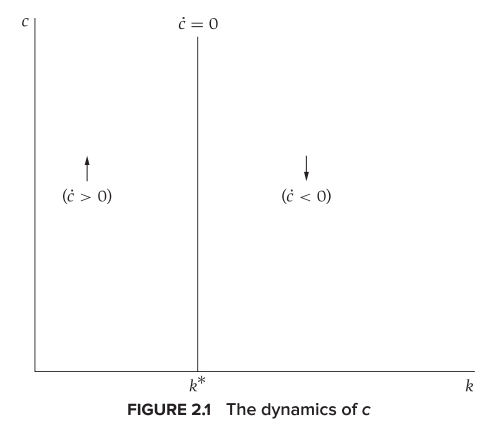
\includegraphics[scale =.5 ]  {figures/Ramsey_C_SS.png}}
\end{figure}








\subsubsection{Dynamics of $ k $}

{\textbf {Derive SS equation (same as what we did in the Solow model):}}

Differentiate $ k = \frac{K}{AL} $ wrt time $ t $,
\begin{align*}
\frac{dK}{dt} = \dot{k}&= \frac{\dot{K}}{AL} - \frac{K}{(AL)^{2}}(\dot{A}L + A \dot{L})
\\
&= \frac{\dot{K}}{AL} - \frac{K}{AL}\frac{\dot{A}}{A} - \frac{K}{AL}\frac{\dot{L}}{L}
\\
&= \frac{Y - CL}{AL} - kg  - kn, \quad \text{given } \dot{K} = Y - CL,\text{ no
depreciation}\\
&= \frac{Y}{AL} - \frac{CL}{L} - (g + n)k, \quad c = \frac{C}{A}\\
\dot{k}&= f(k) - c - (g + n)k, \quad Y = F(K,AL) = ALF(\frac{K}{AL},1)
\end{align*}
So, we receive
\begin{equation*}
\dot{k}= f(k) - c - (g + n)k.
\end{equation*}
Note, $ I = Y - C $. 

So, the above equation shows that $ \dot{k} $ is the difference between actual 
investment per effective labor, $ f(k) - c $, and break-even investment per effective
labor, $ (g + n)k $.

Rewrite the equaiton we receive the SS equation. For a given $ k $, the consumption
$ c $ that implies $ \dot{k} = 0 $ is given by
\begin{equation*}
c = f(k) - (g + n)k
\end{equation*}
When $ c $ exceeds the above level, $ \dot{k} < 0 $, $ k $ will decrease.\\
When $ c $ is below this level, $ \dot{k} > 0 $, $ k $ will increase.\\
When $ k $ is sufficiently large, $ \dot{k} < 0 $ for any $ c > 0 $.

\begin{figure}[H]
\center{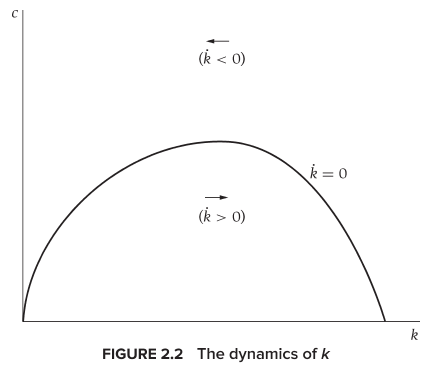
\includegraphics[scale =.6 ]  {figures/Ramsey_k_SS.png}}
\end{figure}



\newpage
{\textbf {Phase diagram:}}


\begin{figure}[ht]
    \centering
    \incfig{phase-diagram}
    \label{fig:phase-diagram}
\end{figure}


In this graph, the SS level of k, $ k ^{*} $ is less than the level of $ k $
which maximizes the $ \dot{k} = 0 $ condition, $ c = f(k) - (g + n)k $ (It is called 
the golden-rule $ k $, $ k_{GR} $).

{\textbf {We draw it in this way because we need to satisfy the transversality 
condition:}}
\begin{equation*}
		\rho - n - (1 - \theta) g > 0
\end{equation*}

{\textbf {Why can can we satisfy this condition by drawing like this?}}
It is because:\\
$ k ^{*} $ is determined by $ \dot{c} = 0 $,
\begin{align*}
		\frac{\dot{c}(t)}{c(t)} &= \frac{f'(k ^{*}) - \rho - \theta g}{\theta} = 0\\
		f'(k ^{*})&= \rho + \theta g
\end{align*}

$ k_{GR} $ is determined by argmax $ \dot{k} = 0 $ condition,
\begin{align*}
\dot{k} &= f(k) - c - (g + n)k\\
c &= f(k) - (g + n)k\\
\frac{\partial c }{\partial k } = f'(k) - (g + n) = 0\\
f'(k_{GR}) = g + n
\end{align*}
Now we receive these two condition for $ k ^{*} $ and $ k_{GR} $:
\begin{align*}
f'(k ^{*}) &= \rho + \theta g\\
f'(k_{GR}) &= g + n
\end{align*}

Recall $ f'(k) < 0 $, therefore, if $ k ^{*} < k_{GR} $, then 
\begin{align*}
\rho + \theta g &> g + n\\
\rho + \theta g  - g - n &> 0\\
\rho - n - (1 - \theta)g &> 0
\end{align*}




The SS level k, $ k ^{*} $ is below $ k_{GR} $ says that the economy does not converge
to the balanced growth path that yields the maximum sustainable level of $ c $.

The SS level k, $ k ^{*} $ is called {\textbf {the modified golden-rule capital stock.}}




\subsection{Shocks}
If there is a drop in $ \rho $, $ \frac{1}{1 + \rho} $ or $ e^{ - \rho t} $ is larger.
It says HH is more impatient. Intuitively, it will increase the SS consumption level.

From two SS conditions:

\begin{align*}
\dot{c}(t) = 0 \rightarrow f'(k ^{*}) &= \rho + \theta g\\
\dot{k}(t) = 0 \rightarrow f'(k ^{*}) &= g + n
\end{align*}
Change in HH time preference will not affect capital accumulation process because
capital evolution is affected by the technology improvement. 

So, $ \dot{k}(t) = 0 $ condition does not change and $ \dot{c}(t) = 0 $ is changed.

Since if $ \rho $ falls, $ \rho + \theta g $ goes down. To hold equation, 
$ f'(k) $ goes down. Since $ f'(\cdot ) < 0 $, $ k ^{*} $ rises.

Hence, if $ \rho $ falls, $ c $ will drop immediately and approach to the stable arm.
Then $ c $ and $ k $ increase gradually.

\begin{figure}[H]
\center{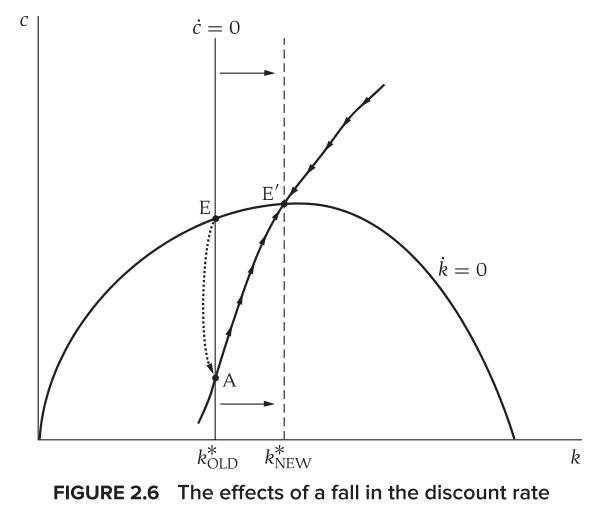
\includegraphics[scale =.5 ]  {figures/shock_in_time_preference.png}}
\end{figure}









\end{document}

